\documentclass[11pt,twoside,b5paper]{article}

\usepackage{xeCJK}
\usepackage{fontspec}
    \setCJKmainfont{Noto Serif CJK TC Light}
    \setCJKmonofont{Noto Serif CJK TC Bold}

\usepackage[vmargin=1in]{geometry}
\pagestyle{empty}

\renewcommand\thesection{\S}
\renewcommand\thesubsection{\arabic{subsection}}
\renewcommand{\arraystretch}{1.1}

\usepackage{amsmath, amsfonts, amssymb, amsthm}
    \newtheorem{ax}{Axiom}
    \newtheorem*{cl}{Corollary}
    \newtheorem*{con}{Conclusion}
    \newtheorem{clm}{Claim}
    \newtheorem{df}{Definition}
    \newtheorem{ex}{Example}
    \newtheorem{exs}{Exercise}
    \newtheorem{lm}{Lemma}
    \newtheorem{pr}{Principle}
    \newtheorem{pp}{Property}
    \newtheorem{pro}{Problem}
    \newtheorem{prop}{Proposition}
    \newtheorem*{rem}{Remark}
    \newtheorem{sol}{Solution}
    \newtheorem{thm}{Theorem}
    \newtheorem{ans}{Answer}

\usepackage{enumerate}
\usepackage{graphicx}
\usepackage{xcolor}
\usepackage{url}
\usepackage{subcaption}
\usepackage[justification=centering]{caption}
\usepackage{float}
\usepackage{multicol}
\usepackage{tikz}
\usetikzlibrary{shapes.geometric, arrows}
\tikzstyle{startstop} = [rectangle, rounded corners, minimum width=1cm, minimum height=1cm,text centered, draw=black]
\tikzstyle{process} = [rectangle, minimum width=1cm, minimum height=1cm, text width=3cm, text centered, draw=black]
\tikzstyle{arrow} = [thick,->,>=stealth]

\begin{document}

\begin{titlepage}
    \section{研究動機}
    
    「Newton's beads \cite{Hooke}」這個現象已被發現多時,也引發眾多教師、知識型網紅爭相解釋成因,然而,除了模糊不清的理論假設和直觀的定性實驗外,未見更深入的定量分析,因此引起我們挑戰解開此現象背後成因的欲望,希望實際利用在高中課程中學習的運動學與基礎程式語言。
    
    \section{研究問題}
    
    \begin{enumerate}
        \item 實際記錄串珠自燒杯下落情形,觀察其最大高度變化的規律性。
        \item 利用VPython編寫符合現實狀況的模擬程式。
        \item 比對程式模擬結果與實驗結果,探討差異,提出成因。
    \end{enumerate}
    
    \section{實驗設備與器材}
    \subsection{實驗器材}
    \begin{enumerate}
        \item 高速攝影機
        \item 腳架
        \item 串珠與燒杯
        \item 游標尺
        \item 捲尺
    \end{enumerate}
    
    \subsection{實驗裝置圖}
    \begin{figure}[H]
        \centering
        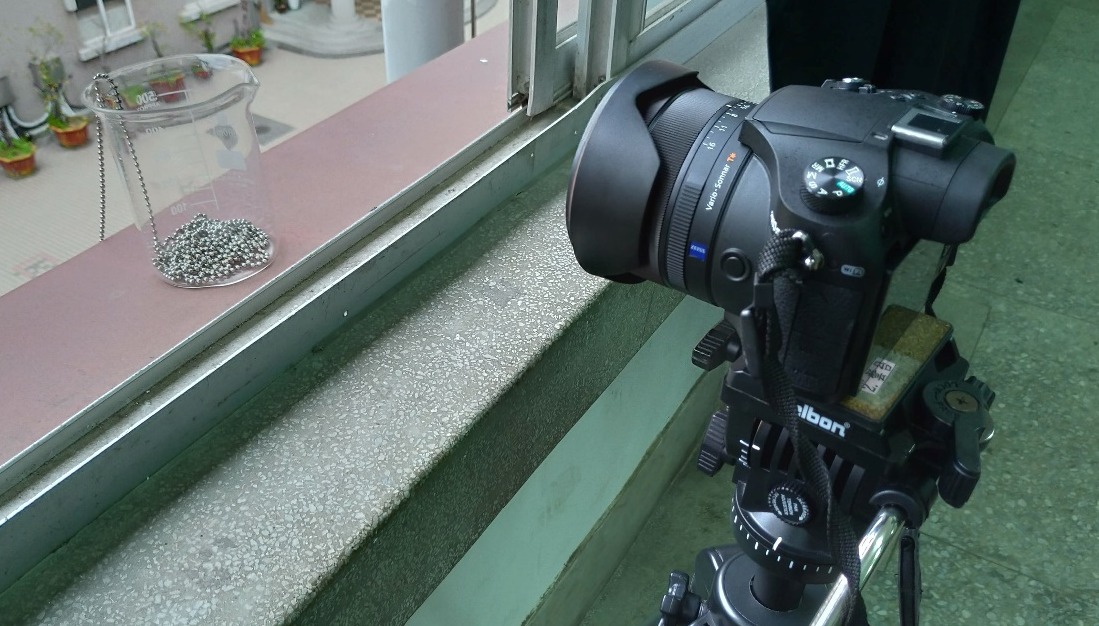
\includegraphics[scale=0.75]{a.png}
    \end{figure}
\end{titlepage}

\section{研究方法與過程}

\subsection{實驗流程圖}
    \begin{figure}[H]
    \centering
    \begin{tikzpicture}[node distance=2cm]
    \node (pro1) [process] {用攝影機拍攝串珠自燒杯落下的情形};
    \node (pro2) [process, below of=pro1] {匯入Tracker,手動追蹤噴起最大高度};
    \node (pro3) [process, below of=pro2]{繪製實驗時間與最大高度關係圖};
    \node (pro4) [process, below of=pro3]{改變施放高度、燒杯半徑等物理量};
    \node (pro5) [process, right of=pro1, xshift=3cm]{用VPython編寫串珠、燒杯模型};
    \node (pro6) [process, below of=pro5]{產出視覺化影像,更改不合理處};
    \node (pro7) [process, below of=pro6]{繪製理論時間與最大高度關係圖};
    \node (pro8) [process, below of=pro7]{考慮更多現實因素(同時得知哪些因素影響串珠噴泉)};
    \draw [arrow] (pro1) -- (pro2);
    \draw [arrow] (pro2) -- (pro3);
    \draw [arrow] (pro3) -- (pro4);
    \draw [arrow] (pro4) -- ++ (-2cm,0) |- node[anchor=west]{} (pro1);
    \draw [arrow] (pro5) -- (pro6);
    \draw [arrow] (pro6) -- (pro7);
    \draw [arrow] (pro7) -- (pro8);
    \draw [arrow] (pro8) -- ++ (2cm,0) |- node[anchor=east]{} (pro5);
    \draw [<->, thick,>=stealth] (pro3) --node[yshift=0.3cm]{比對} (pro7);
    \draw [arrow] (2.5,-4) |- (pro8);
    \end{tikzpicture}
\end{figure}

\subsection{實驗方法}
    \begin{enumerate}
        \item 將燒杯放在足夠高的大樓圍牆邊(樓高大於串珠長),雙手扶持,架設攝影機,調整至觀察串珠噴起之最佳觀察視野。
        \item 施放串珠,同時啟動攝影,紀錄串珠噴起狀態。
        \item 將影片匯入Tracker ,手動追蹤串珠噴起最高點。
        \item 利用燒杯高度為比例尺,由Tracker繪製噴起高度與時間之關係圖。
    \end{enumerate}
    
\subsection{程式編寫}
    \begin{enumerate}
        \item 由VPython編寫符合現實狀況之程式,顯示視覺化影像。
        \item 觀察程式模擬影像,修改不合理處與相關物理量。
    \end{enumerate}
\subsection{程式與理論比較}
\begin{enumerate}
    \item 比較Tracker分析的實驗結果與VPython程式模擬結果。
    \item 針對不同處重新改良程式,若模擬情況更加接近真實結果,則可得知影響串出噴起的因素。
\end{enumerate}

\section{研究結果}

\subsection{實驗結果:串珠噴起最高點高度與時間(三次實驗)}

串珠參數如下:
\begin{table}[H]
    \centering
    \begin{tabular}{c|c|c}
    長度(m) & 重量(g) & 線密度(g/m) \\
    4.532 & 78.8 & 17.39
    \end{tabular}
\end{table}

\begin{figure}[H]
    \centering
    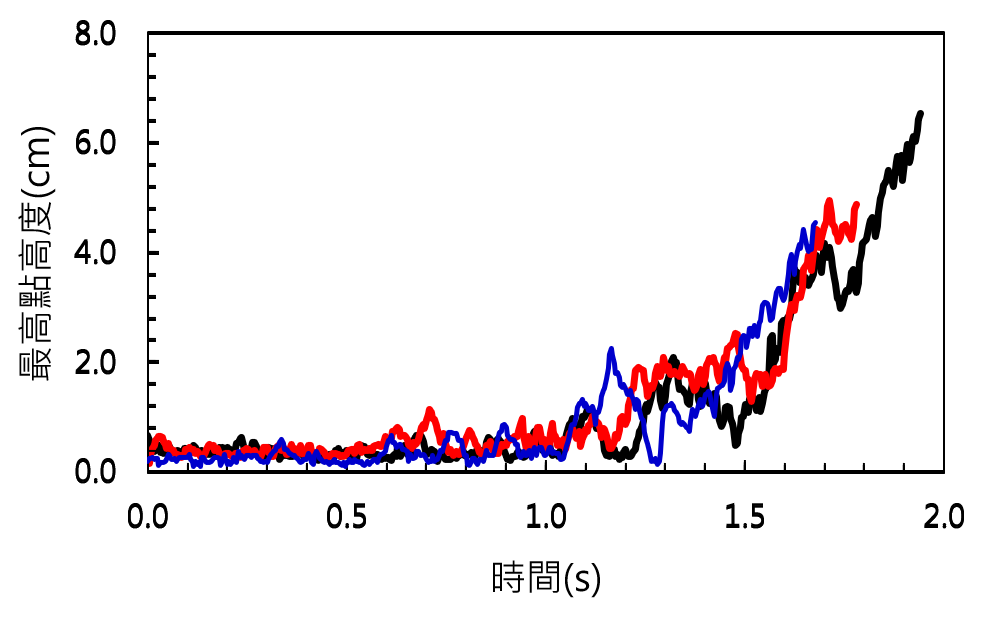
\includegraphics[scale=0.5]{b.PNG}
\end{figure}

三次實驗結果呈現一致的趨勢,包括:

\begin{enumerate}
    \item 0.5秒末前無明顯噴起。
    \item 0.5秒末左右後規律性噴起,約0.5-1.0公分。
    \item 1秒末左右後有大幅度的噴起,約2.0公分,之後噴起高度持續增加,超過4.5公分。
    \item 從規律性噴起到落完約1.1-1.3秒。
\end{enumerate}

\subsection{模擬原理}

\subsubsection{虎克定律 \cite{Hooke}}
    一根長度為$L$、橫截面積$A$的稜柱形棒,在力學上都可以用虎克定律來模擬—其單位伸長(或縮減)量$\varepsilon$(應變)在常係數$Ε$(彈性模量)下,與拉(或壓)應力$\sigma$成正比例,即:
    \[
        \Delta L=\frac{1}{E}\times L\times \sigma
    \]
    虎克定律應用的一個常見例子是彈簧。在彈性限度內,彈簧的彈力F和彈簧的長度變化量$x$成線性關係,即:
    \[
        F=-kx
    \]
    其中$k$是彈簧的勁度係數(彈力係數),由材料性質、幾何外形決定。負號象徵彈簧產生的彈力與其伸長(壓縮)的方向相反,這種彈力稱為回復力,表示它有使系統回復平衡的趨勢。

\subsubsection{	碰撞與彈性係數 \cite{Re}}

一維碰撞案例,則所有的速度都是純量。設定坐標軸為$x$軸,與正$x$軸同方向的運動的速度為正值,反方向的運動的速度為負值。恢復係數$e$可以表達為:
    \[
        e=\frac{v_{2f}-v_{1f}}{v_{1i}-v_{2i}}.
    \]

其中,$v_{1i}$、$v_{1f}$、$v_{2i}$、$v_{2f}$ 分別是一個物體、第二個物體在碰撞前和碰撞後的速度。假設一個物體碰撞的另一個物體是固定不動,像地板、牆壁,則恢復係數$e$為:
\[
    e=\frac{v_f}{v_i}
\]

其中,$v_i$是碰撞前的速率,$v_f$是碰撞後的速率。

\subsubsection{Python中陣列與迴圈的運算速度比較 \cite{Py} }

在Python中使用陣列(array)比使用迴圈(for)運算速度更快。同樣運算100000組數字相乘,答案都正確的情況下,使用迴圈比使用陣列多運算約7.3倍的時間。

\subsection{模擬結果}

\subsubsection{直線形模型}

\begin{figure}[H]
    \centering
    \begin{subfigure}[t]{0.3\linewidth}
    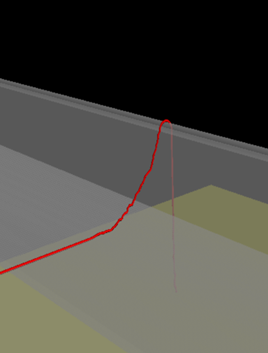
\includegraphics[height=4cm]{1.png}
    \end{subfigure}
    \begin{subfigure}[t]{0.65\linewidth}
    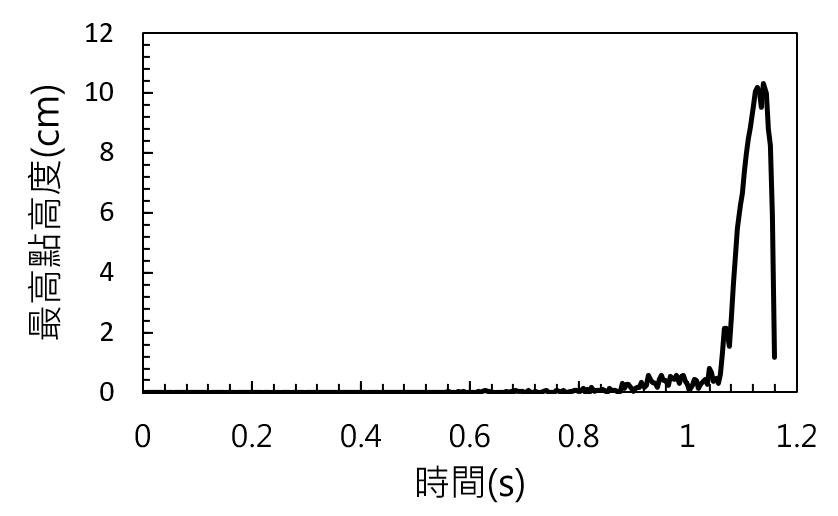
\includegraphics[height=4cm]{1a.PNG}
    \end{subfigure}
\end{figure}

此模型無法適度顯示串珠自燒杯下落的情形,只有在快結束時有大幅度噴起。

\subsubsection{環形模型}

\begin{figure}[H]
    \centering
    \begin{subfigure}[t]{0.3\linewidth}
    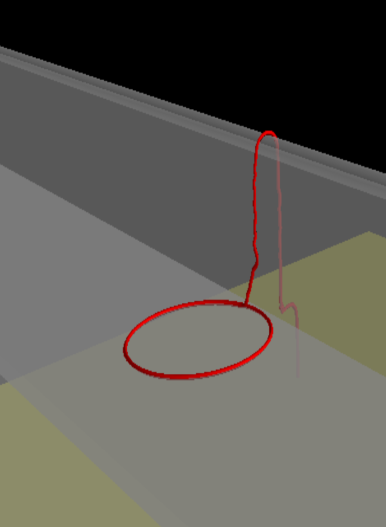
\includegraphics[height=4cm]{2.png}
    \end{subfigure}
    \begin{subfigure}[t]{0.65\linewidth}
    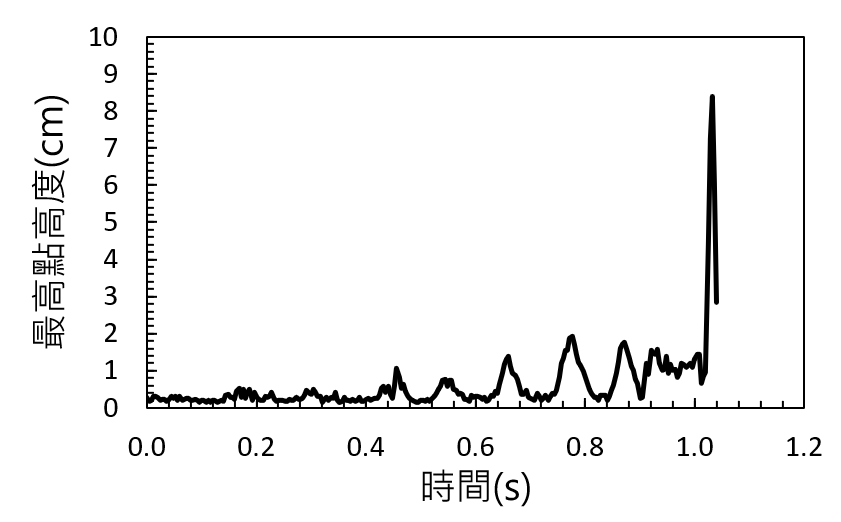
\includegraphics[height=4cm]{2b.PNG}
    \end{subfigure}
\end{figure}

當模型內將串珠盤起時,在中期出現規律的噴起,但噴起時間比真實情況短。

\section{討論}

\subsection{串珠噴起前期沒有明顯噴起的原因}
串珠下落時將位能轉換為動能,再藉由彼此連結將動能傳遞到上方串珠,而上方串珠將動能傳換為位能,使串珠噴起,而此時期由於下落距離不夠長,所以沒有足夠多的能量傳遞至上方,是故沒有明顯噴起。

\subsection{串珠噴起中期有規律性明顯噴起的原因}
當串珠達到足夠速度時,由於杯內串珠繞在杯底,當串珠拉起,消耗杯底串珠時,有相對速度朝向杯壁或遠離杯壁,使得杯內被拉起的串珠與杯外落下的串珠速度不一致。當相對速度朝向杯壁時,杯內被拉起的串珠之速度大於杯外落下的串珠速度,從而使串珠堆積在杯緣處;當相對速度遠離杯壁時,杯內被拉起的串珠之速度小於於杯外落下的串珠速度,從而消耗串珠在杯緣處堆積,如此反覆作用的結果導致中期有規律性的噴起。

\subsection{串珠噴起末期有大幅度噴起的原因}
此時留在杯底的串珠甚少,已無中期的「纏繞」,而是相當於一條一端繫重物的繩子將另一端留在燒杯內,當「重物」下墜時,另一端重量甚小,被快速拉起,又由於慣性作用,速度垂直分量持續將繩末帶往高處,形同「甩尾」。

\subsection{}
因為實驗時礙於高速攝影機僅能錄製3秒的限制,所以我們當串珠開始穩定下落時才開始錄製,因此此實驗數據無法精確顯示串珠自靜止開始到完全落下的時間,故此模擬結果之時間經平移過,將穩定噴起的開始時間設置與實驗相似。

\subsection{}
在模擬過程中,相同程式碼用不同的兩臺電腦會產生差異相當大的結果(見下圖)。我們認為是因為此串珠是用「複擺」為單位寫成的,因此屬於混沌系統,不同電腦間的微小浮點數誤差導致截然不同的曲線。

\begin{figure}[H]
    \centering
    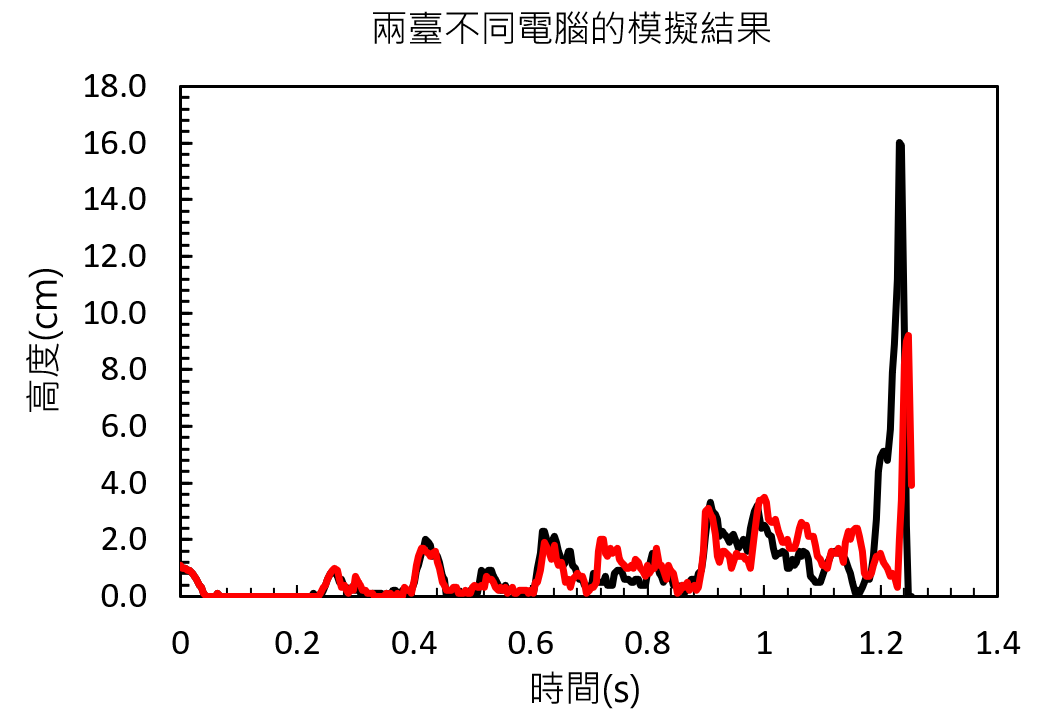
\includegraphics[scale=0.5]{3.PNG}
\end{figure}

\section{結論}

\subsection{程式結果與實驗結果大致一致,可將串珠下落時期分為}
\begin{enumerate}
    \item 前期:能量累積期。此時期未有足夠下方位能傳換為上方位能,是故無明顯噴起。 
    \item 中期:規律噴發期。此時期有足夠動能,同時藉由燒杯內之纏繞,呈現規律的噴起。
    \item 末期:慣性甩尾期。此時期已無串珠在杯底糾纏,而是如同一端繫重的繩子,將杯底殘餘串珠快速拉起。
\end{enumerate}

\subsection{未來展望}
\begin{enumerate}
    \item 程式模擬結果與實驗結果呈現相同趨勢,然而噴起時間略短,參閱論文後,推測應為程式未考量串珠基本性質,導致能量在不合理處消耗、力的傳遞不符合真實狀況,未來將在程式中增加串珠的基本性質。
    \item 改變實驗時串珠的長度、線密度、釋放高度等參數,期望能推論出影響此現象在中期穩定噴發時的因素。
    \item 此程式只要略加更變初始條件,即可模擬任何有關繩、串珠的科學問題。
    \item 利用統計方式探討不同變因下,此混沌系統所模擬出的變化趨勢。
\end{enumerate}

\medskip
\renewcommand{\refname}{\S\quad 參考資料}
\nocite{*}
\bibliographystyle{unsrt}
\bibliography{Reference.bib}

\end{document}